% !TEX root = ./document.tex

\documentclass[a4paper, spanish]{article}

\usepackage{mystyle}
\usepackage{myvars}

\begin{document}

  \maketitle

  \begin{itemize}
    \item \textbf{Archivo}: \texttt{NE2.txt}
    \item \textbf{Serie}: Número de espectadores de cine por meses desde Enero de 1984 a Diciembre de 2000.
  \end{itemize}

  \section{Ajustar por mínimos cuadrados un modelo con tendencia más ondas a la serie escribiendo explícitamente las ecuaciones de las ondas incluidas en el modelo. Añadir la descripción completa de la serie residual.}

    \paragraph{}
    Tal y como se indica al comienzo del documento, en este trabajo se va a tratar de ajustar una serie referida al número de espectadores de cine por meses dese Enero del año $1984$ hasta Diciembre del año $2000$. Esto se corresponde con un total de $204$ observaciones mensuales. La serie completa recoge información de $204 / 12 = 17$ años acerca del número de espectadores.

    \begin{figure}[h]
      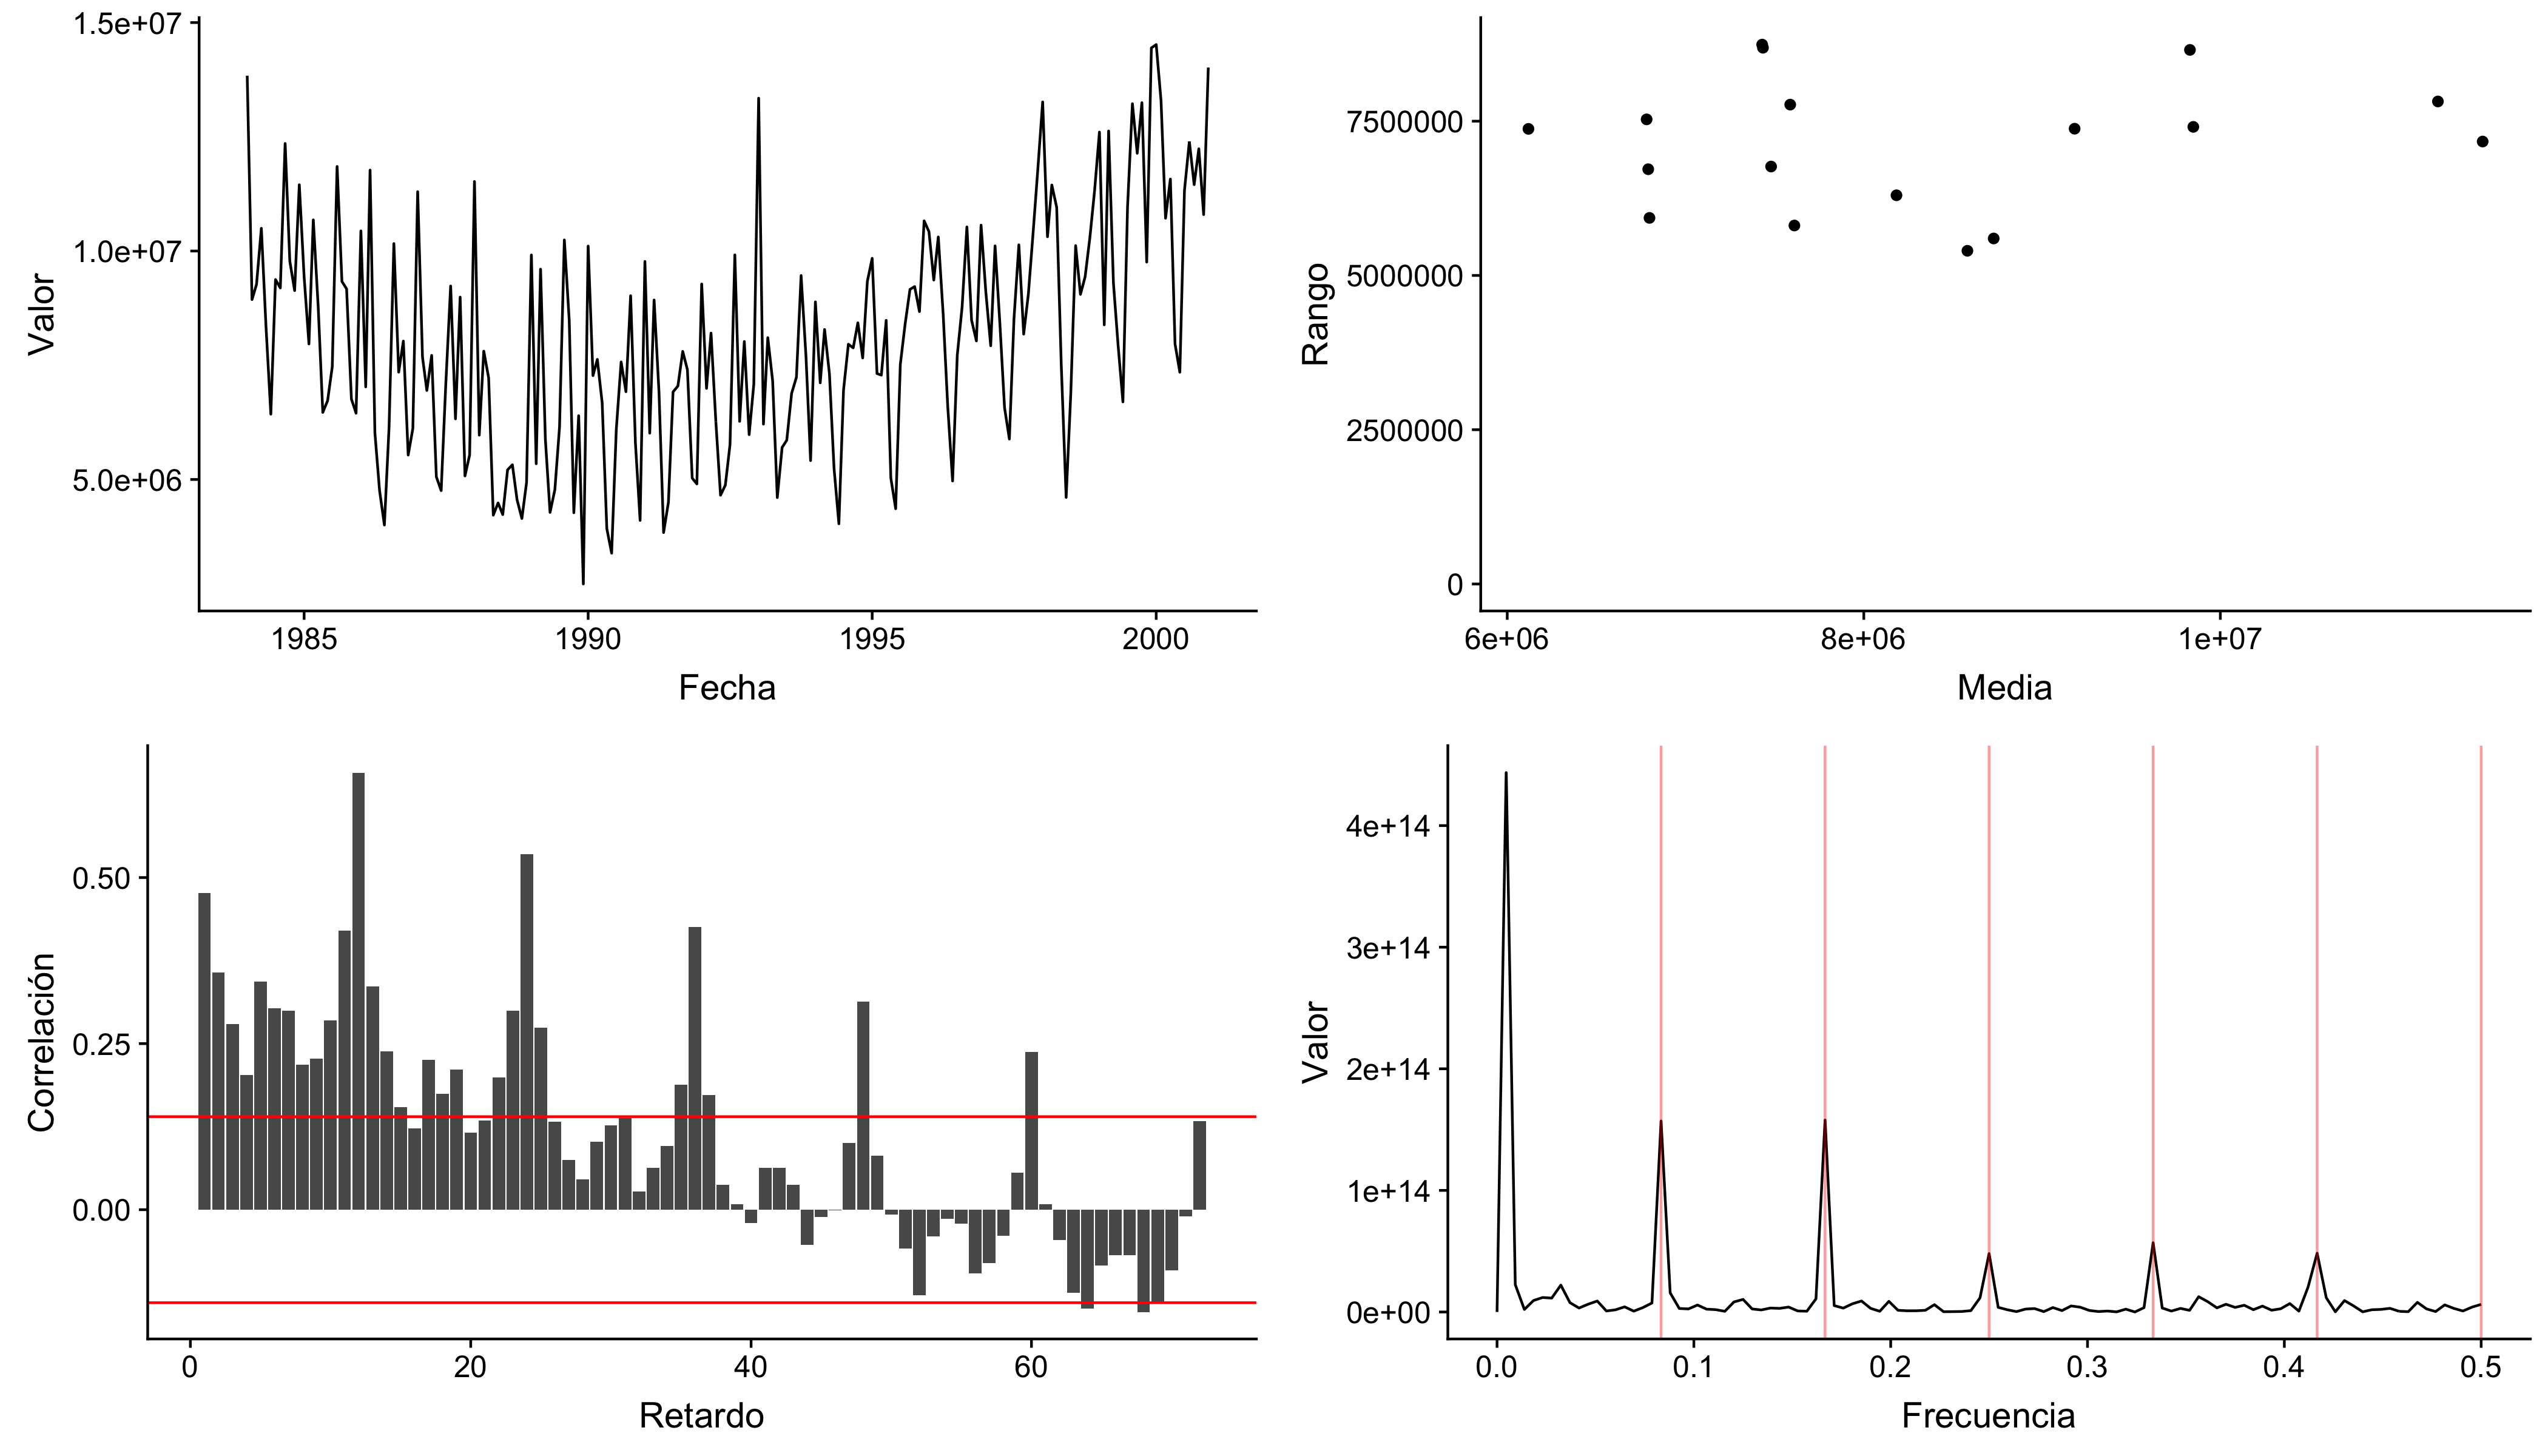
\includegraphics[width=\linewidth]{espectadores}
      \caption{Gráfico de la serie, Diagrama de Dispersión, Correlograma y Periodograma de la serie \emph{Espectadores}.}
      \label{fig:espectadores}
    \end{figure}

    \paragraph{}
    El primer paso antes de realizar ningún ajuste sobre la serie es conocer la estructura de la misma, lo cual permitirá entender mejor su comportamiento facilitando la realización de una modelización más coherente. Por tanto, en la figura \ref{fig:espectadores} se muestra el gráfico de la serie, el gráfico de dispersión \emph{rango-media}, el correlograma y el periodograma de la misma respectivamente.

    \paragraph{}
    Lo más notable en la estructura de la serie es su marcada tendencia parabólica, con su mínimo en torno a los años \emph{1990}. Esto nos será de gran ayuda para modelizar la serie, utilizando una modelización cuadrática para la componente de tendencia. También parece verse una componente estacional, que es difícil de estudiar directamente debido a la tendencia. Sin embargo, esta se puede ver bien en el periodograma y correlograma, los cuales comentaremos posteriormente.

    \paragraph{}
    En cuanto al diagrama de dispersión \emph{rango-media}, este ha sido generado realizando agrupaciones de longitud igual a la estacionalidad ($12$ meses). En este gráfico no parece que haya una relación fuerte entre dichas variables. Esto se intuye debido a la pendiente nula que se puede apreciar en el gráfico.

    \paragraph{}
    En cuanto al correlograma, en este se aprecia la estructura de correlaciones que indica una componente de tendencia fuertemente marcada. Esta se aprecia en las correlaciones múltiplos de la estacionalidad. Es decir, aquellas correlaciones tales que $12 \ mod \ i = 0$. Si nos fijamos únicamente en estas, podemos apreciar un decricimiento marcademente lineal, lo cual nos confirma la existencia de una componente estacional.

    \paragraph{}
    En cuanto al periodograma, se vuelve a confirmar la idea que acabamos de indicar en el anterior párrafo: La serie tiene una marcada estacionalidad de periodo 12. En este caso queda reflejado en la forma determinista en que las frecuencias de la forma $i/12$ con $i \in \{1, 2, ..., 6\}$ destacan sobre el resto, en especial las dos primeras.

    \paragraph{}
    Una vez descrita la serie, estamos en condiciones suficientes para realizar un ajuste sobre la serie. En este caso la modelización de la tendencia se realizará basandose en un modelo con tendencia (cuadrática) + ondas. Esto lo haremos en dos fases, inicialmente ajustaremos un modelos con todas las ondas posibles, cuyo resultado deberá ser totalmente equivalente al modelo basado en índices que se ajusta en el segundo apartado. Posteriormente, para reducir la complejidad del modelo, eliminaremos aquellas componentes de la onda que no resulten significativos para explicar el modelo.

    \paragraph{}
    En cuanto a la componente de la tendecia de la serie, ajustaremos un modelo basado en en regresión polinómica de segundo orden, esto es $E[Y_t] = \beta_0 + \beta_1 \cdot t + \beta_2 t ^ 2$ (nótese que no se ha indicado el error aleatorio dado que se ha modelizado respecto del valor esperado). En este modelo utilizaremos como origen la observación $0$, por lo tanto, para predecir el valor esperado para la observación $t + 1$ deberemos utilizar el índice $t + 1$.

    \paragraph{}
    En cuanto a la modelización de la tendencia, esta se basará en una modelización de ondas como sumas de senos y cosenos con frecuencia angular $\omega_i = \frac{2 \pi i}{12}$ con $i \in \{1, ..., 6\}$. Esto se debe a que la estacionalidad de la serie es de periodo $s = 12$ y por tanto el número de armónicos que podemos utilizar es $s / 2$. Por tanto, en este caso $12 / 2 = 6$. Por lo tanto, la componente regresora basada en ondas será de la forma $\gamma_{i,1} cos\left(\frac{2 \pi  i}{12} t\right) + \gamma_{i,2} sin\left(\frac{2 \pi i}{12} t\right)$ para la componente estacional $i$-ésima y la observación $t$-ésima. Es importante darse cuenta de que el $sin(\pi t) = 0$ para todo $t$ entero, por lo que ignoraremos dicho regresor en el modelo.

    \paragraph{}
    Entonces, nuestro modelo requiere de la estimación de $3$ parámetros referidos a la componente de tendencia y $6 + 6 -1 = 11$ parámetros referidos a la componente de estacionalidad. Esto nos da un total de $3 + 11 = 14$ parámetros a estimar para tener bien definido el modelo. A continuación se indica el modelo completo:

    \begin{align*}
      E[X_{n + k}] = \beta_0 &+ \beta_1 \cdot (n + k) + \beta_2 \cdot(n + k) \\
      &+ \gamma_{1,1} cos\left(\frac{2 \pi  }{12} t\right) + \gamma_{1,2} sin\left(\frac{2 \pi  }{12} t\right) \\
      &+ \gamma_{2,1} cos\left(\frac{2 \pi 2}{12} t\right) + \gamma_{2,2} sin\left(\frac{2 \pi 2}{12} t\right) \\
      &+ \gamma_{3,1} cos\left(\frac{2 \pi 3}{12} t\right) + \gamma_{3,2} sin\left(\frac{2 \pi 3}{12} t\right) \\
      &+ \gamma_{4,1} cos\left(\frac{2 \pi 4}{12} t\right) + \gamma_{4,2} sin\left(\frac{2 \pi 4}{12} t\right) \\
      &+ \gamma_{5,1} cos\left(\frac{2 \pi 5}{12} t\right) + \gamma_{5,2} sin\left(\frac{2 \pi 5}{12} t\right) \\
      &+ \gamma_{6,1} cos\left(\frac{2 \pi 6}{12} t\right)
    \end{align*}


    \begin{table}
      \centering
      \begin{tabular}{l|c|c|c|c}%
          \bfseries Parámetro & Valor & Error & T & pvalor
          \csvreader[head to column names]{res/data/ondascompletasparams.csv}{}
          {\\\hline\PARM & \VALUE & \STDERR & \T & \P}
      \end{tabular}
      \caption{Parámetros ajustados para el modelo basado en ondas con todos los armónicos.}
      \label{table:waves_complete_params}
    \end{table}

    \paragraph{}
    Por lo tanto se ha procedido al ajuste de dicho modelo, el cual se muestran en la tabla \ref{table:waves_complete_params}. Analizando los p-valores (referidos al test acerca de si pueden ser considerados nulos), podemos ver que $\gamma_{1, 2}$ y  $\gamma_{3,2}$ no rechazan dicha hipótesis. Si visualizamos el modelo, estos se refieren a $sin\left(\frac{2 \pi  }{12} t\right)$ y $sin\left(\frac{2 \pi 3}{12} t\right)$ respectivamente. Por lo tanto, vamos a realizar un nuevo ajuste sobre el modelo sin dichos regresores:

    \begin{align*}
      E[X_{n + k}] = \beta_0 &+ \beta_1 \cdot (n + k) + \beta_2 \cdot(n + k) \\
      &+ \gamma_{1,1} cos\left(\frac{2 \pi  }{12} t\right) \\
      &+ \gamma_{2,1} cos\left(\frac{2 \pi 2}{12} t\right) + \gamma_{2,2} sin\left(\frac{2 \pi 2}{12} t\right) \\
      &+ \gamma_{3,1} cos\left(\frac{2 \pi 3}{12} t\right) \\
      &+ \gamma_{4,1} cos\left(\frac{2 \pi 4}{12} t\right) + \gamma_{4,2} sin\left(\frac{2 \pi 4}{12} t\right) \\
      &+ \gamma_{5,1} cos\left(\frac{2 \pi 5}{12} t\right) + \gamma_{5,2} sin\left(\frac{2 \pi 5}{12} t\right) \\
      &+ \gamma_{6,1} cos\left(\frac{2 \pi 6}{12} t\right)
    \end{align*}

    \paragraph{}
    En este caso, los parámetros ajustados se muestran en la tabla \ref{table:waves_params}. Tal y como podemos apreciar en este caso todos los pvalores indican que los parámetros son significativamente distintos de cero (tomando un nivel de confianza del $90\%$). Entonces, procederemos al análisis de la serie residuales obtenidos para tratar de confirmar el ajuste del modelo. Para ello debemos confirmar que esta serie se refiere a un ruido blanco (no existe correlacion entre las distintas observaciones, su media es cero y su varianza constante).

    \begin{table}
      \centering
      \begin{tabular}{l|c|c|c|c}%
          \bfseries Parámetro & Valor & Error & T & pvalor
          \csvreader[head to column names]{res/data/ondassignificativasparams.csv}{}
          {\\\hline\PARM & \VALUE & \STDERR & \T & \P}
      \end{tabular}
      \caption{Parámetros ajustados para el modelo basado en ondas con armónicos significativos.}
      \label{table:waves_params}
    \end{table}

    \paragraph{}
    [TODO]

    \paragraph{}
    Al igual que se ha indicado anteriormente para el caso de la serie original, en este caso se incluyen un conjunto de diagramas sobre la serie de residuales, la cual se muestra en la figura \ref{fig:residuals}.

    \begin{figure}
      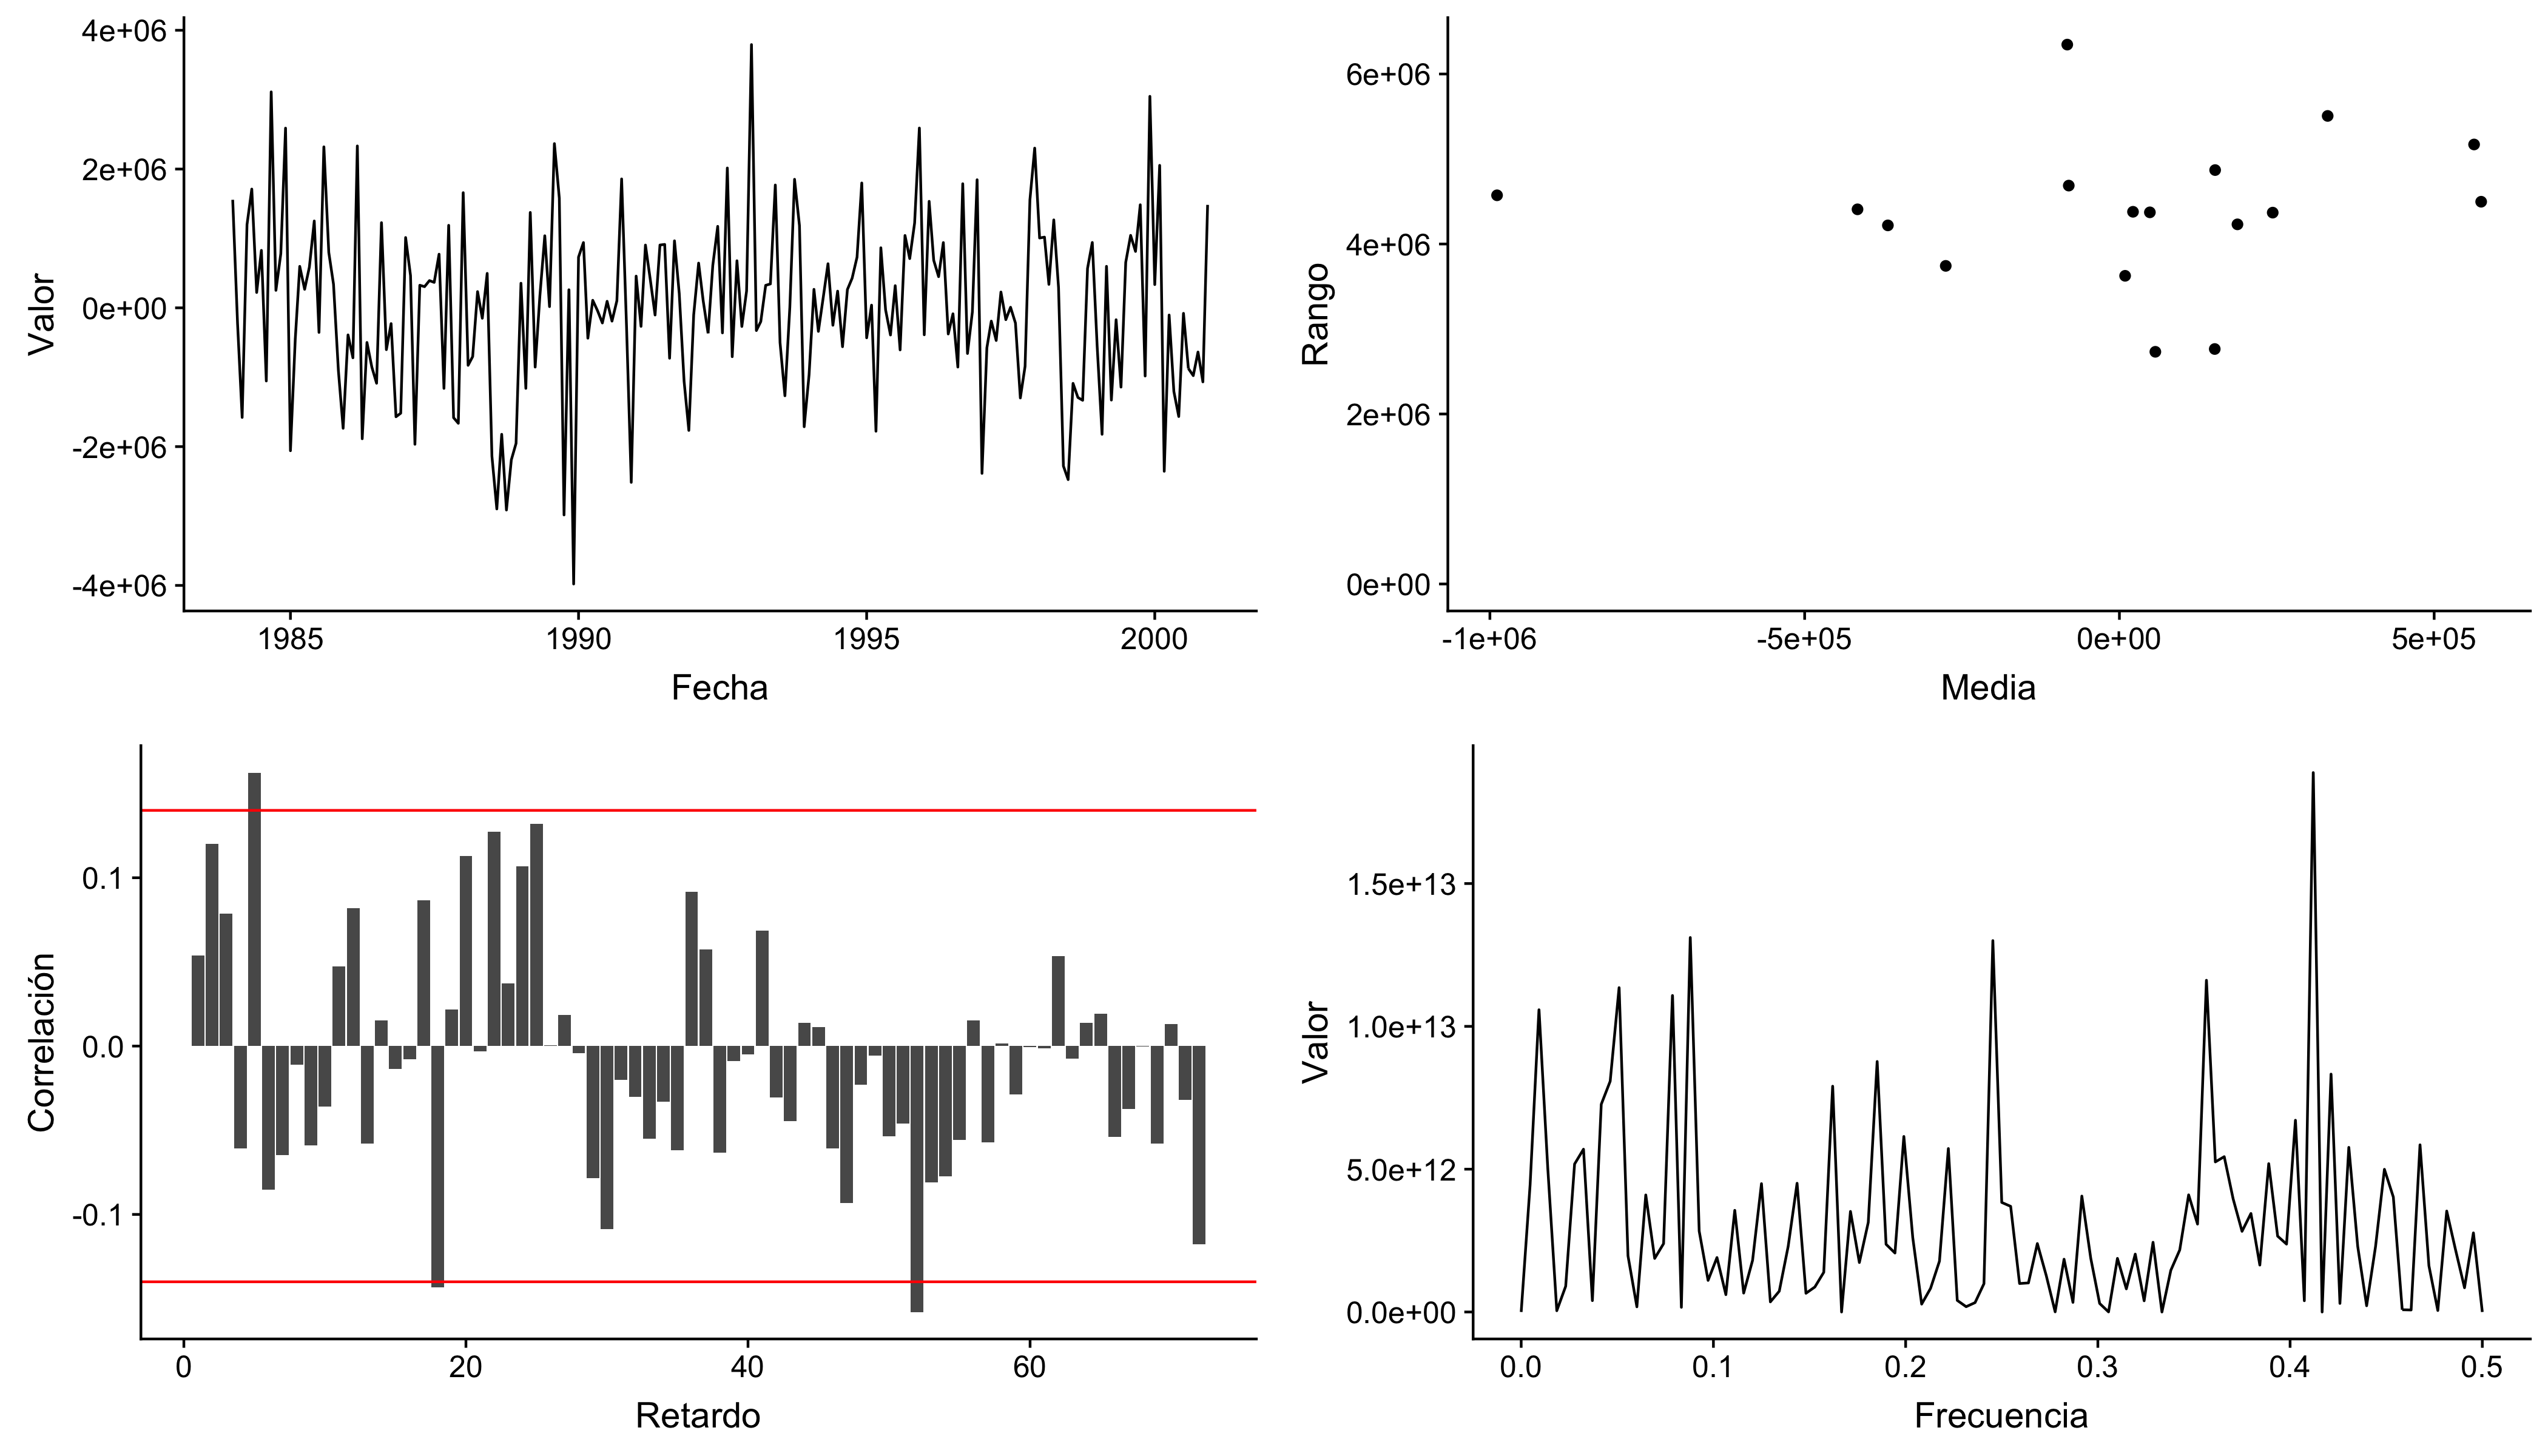
\includegraphics[width=\linewidth]{residuos}
      \caption{Gráfico de la serie, Diagrama de Dispersión, Correlograma y Periodograma de la serie de residuales tras el ajuste del modelo}
      \label{fig:residuals}
    \end{figure}

    \paragraph{}
    [TODO]


  \section{Ajustar por mínimos cuadrados un modelo con tendencia más índices estacionales a la serie y comentar diferencias con el ajuste anterior.}

    \paragraph{}
    [TODO]


    \begin{align*}
      E[X_{n + k}] = \beta_0 &+ \beta_1 \cdot (n + k) + \beta_2 \cdot(n + k) \\
      &+ \gamma_{1} S_{1} + \gamma_{2} S_{2}  + \gamma_{3} S_{3} + \gamma_{4} S_{4} \\
      &+ \gamma_{5} S_{5} + \gamma_{6} S_{6}  + \gamma_{7} S_{7} + \gamma_{8} S_{8} \\
      &+ \gamma_{9} S_{9} + \gamma_{10} S_{10}  + \gamma_{11} S_{11}
    \end{align*}

    \paragraph{}
    [TODO]

    \begin{table}
      \centering
      \begin{tabular}{l|c|c|c|c}%
          \bfseries Parámetro & Valor & Error & T & pvalor
          \csvreader[head to column names]{res/data/indicesparams.csv}{}
          {\\\hline\PARM & \VALUE & \STDERR & \T & \P}
      \end{tabular}
      \caption{Parámetros ajustados para el modelo basado en índices.}
      \label{table:indices_params}
    \end{table}

    \paragraph{}
    [TODO]

\end{document}
